\documentclass{standalone}
\usepackage{tikz}
\usetikzlibrary{patterns, positioning}


\begin{document}
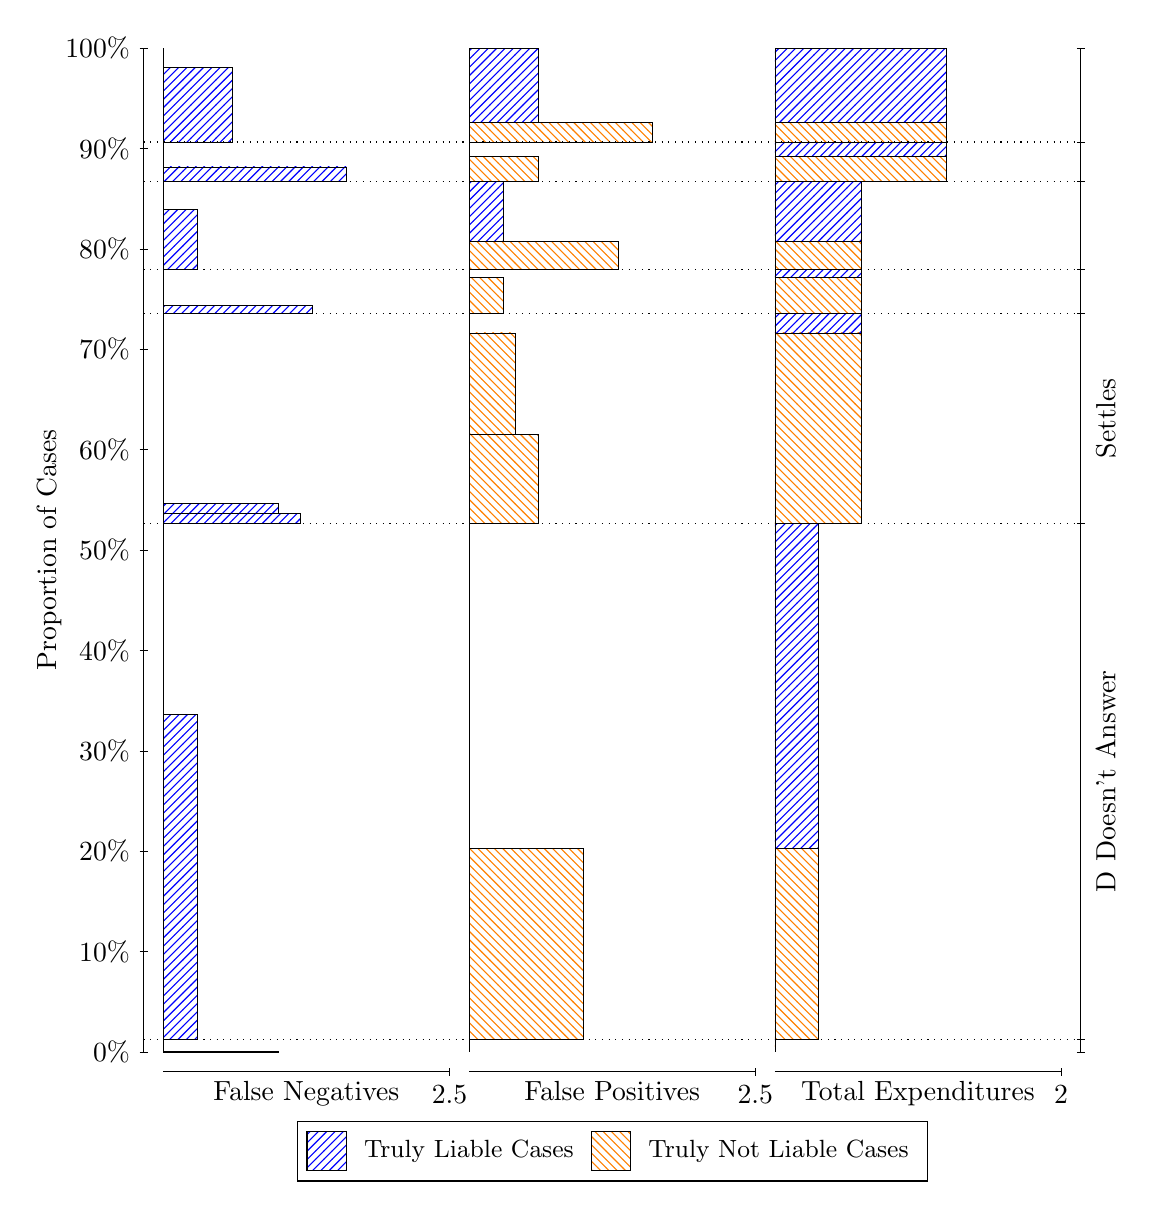
\begin{tikzpicture}
\draw[black, very thin] (1.5,1.75) -- (1.5,14.5);
\node[rotate=90, text=black, anchor=center] at (0.3, 8.125) {Proportion of Cases};
\draw[black, very thin] (1.45,1.75) -- (1.55,1.75);
\node[text=black, anchor=east] at (1.45, 1.75) {0\%};
\draw[black, very thin] (1.45,3.025) -- (1.55,3.025);
\node[text=black, anchor=east] at (1.45, 3.025) {10\%};
\draw[black, very thin] (1.45,4.3) -- (1.55,4.3);
\node[text=black, anchor=east] at (1.45, 4.3) {20\%};
\draw[black, very thin] (1.45,5.575) -- (1.55,5.575);
\node[text=black, anchor=east] at (1.45, 5.575) {30\%};
\draw[black, very thin] (1.45,6.85) -- (1.55,6.85);
\node[text=black, anchor=east] at (1.45, 6.85) {40\%};
\draw[black, very thin] (1.45,8.125) -- (1.55,8.125);
\node[text=black, anchor=east] at (1.45, 8.125) {50\%};
\draw[black, very thin] (1.45,9.4) -- (1.55,9.4);
\node[text=black, anchor=east] at (1.45, 9.4) {60\%};
\draw[black, very thin] (1.45,10.675) -- (1.55,10.675);
\node[text=black, anchor=east] at (1.45, 10.675) {70\%};
\draw[black, very thin] (1.45,11.95) -- (1.55,11.95);
\node[text=black, anchor=east] at (1.45, 11.95) {80\%};
\draw[black, very thin] (1.45,13.225) -- (1.55,13.225);
\node[text=black, anchor=east] at (1.45, 13.225) {90\%};
\draw[black, very thin] (1.45,14.5) -- (1.55,14.5);
\node[text=black, anchor=east] at (1.45, 14.5) {100\%};

\draw[black, very thin] (13.4,1.75) -- (13.4,14.5);
\draw[black, very thin] (13.35,1.75) -- (13.45,1.75);
\node[anchor=west] at (13.35, 1.75) {};
\draw[black, very thin] (13.35,1.9102) -- (13.45,1.9102);
\node[anchor=west] at (13.35, 1.9102) {};
\draw[black, very thin] (13.35,8.4642) -- (13.45,8.4642);
\node[anchor=west] at (13.35, 8.4642) {};
\draw[black, very thin] (13.35,11.132) -- (13.45,11.132);
\node[anchor=west] at (13.35, 11.132) {};
\draw[black, very thin] (13.35,11.686) -- (13.45,11.686);
\node[anchor=west] at (13.35, 11.686) {};
\draw[black, very thin] (13.35,12.805) -- (13.45,12.805);
\node[anchor=west] at (13.35, 12.805) {};
\draw[black, very thin] (13.35,13.306) -- (13.45,13.306);
\node[anchor=west] at (13.35, 13.306) {};
\draw[black, very thin] (13.35,14.5) -- (13.45,14.5);
\node[anchor=west] at (13.35, 14.5) {};

\draw[black, very thin, pattern color=blue, pattern=north east lines] (1.75,1.75) rectangle (3.2033,1.7594);
\draw[black, very thin, pattern color=orange, pattern=north west lines] (1.75,1.7594) rectangle (1.75,1.9102);
\draw[black, very thin, pattern color=blue, pattern=north east lines] (1.75,1.9102) rectangle (2.186,6.0356);
\draw[black, very thin, pattern color=orange, pattern=north west lines] (1.75,6.0356) rectangle (1.75,8.4642);
\draw[black, very thin, pattern color=blue, pattern=north east lines] (1.75,8.4642) rectangle (3.494,8.587);
\draw[black, very thin, pattern color=blue, pattern=north east lines] (1.75,8.587) rectangle (3.2033,8.713);
\draw[black, very thin, pattern color=orange, pattern=north west lines] (1.75,8.713) rectangle (1.75,11.132);
\draw[black, very thin, pattern color=blue, pattern=north east lines] (1.75,11.132) rectangle (3.6393,11.227);
\draw[black, very thin, pattern color=orange, pattern=north west lines] (1.75,11.227) rectangle (1.75,11.686);
\draw[black, very thin, pattern color=blue, pattern=north east lines] (1.75,11.686) rectangle (2.186,12.451);
\draw[black, very thin, pattern color=orange, pattern=north west lines] (1.75,12.451) rectangle (1.75,12.805);
\draw[black, very thin, pattern color=blue, pattern=north east lines] (1.75,12.805) rectangle (4.0753,12.99);
\draw[black, very thin, pattern color=orange, pattern=north west lines] (1.75,12.99) rectangle (1.75,13.306);
\draw[black, very thin, pattern color=blue, pattern=north east lines] (1.75,13.306) rectangle (2.622,14.251);
\draw[black, very thin, pattern color=orange, pattern=north west lines] (1.75,14.251) rectangle (1.75,14.5);
\draw[black, very thin, pattern color=orange, pattern=north west lines] (5.6333,1.75) rectangle (5.6333,1.9008);
\draw[black, very thin, pattern color=blue, pattern=north east lines] (5.6333,1.9008) rectangle (5.6333,1.9102);
\draw[black, very thin, pattern color=orange, pattern=north west lines] (5.6333,1.9102) rectangle (7.0867,4.3388);
\draw[black, very thin, pattern color=blue, pattern=north east lines] (5.6333,4.3388) rectangle (5.6333,8.4642);
\draw[black, very thin, pattern color=orange, pattern=north west lines] (5.6333,8.4642) rectangle (6.5053,9.5896);
\draw[black, very thin, pattern color=orange, pattern=north west lines] (5.6333,9.5896) rectangle (6.2147,10.883);
\draw[black, very thin, pattern color=blue, pattern=north east lines] (5.6333,10.883) rectangle (5.6333,11.132);
\draw[black, very thin, pattern color=orange, pattern=north west lines] (5.6333,11.132) rectangle (6.0693,11.59);
\draw[black, very thin, pattern color=blue, pattern=north east lines] (5.6333,11.59) rectangle (5.6333,11.686);
\draw[black, very thin, pattern color=orange, pattern=north west lines] (5.6333,11.686) rectangle (7.5227,12.04);
\draw[black, very thin, pattern color=blue, pattern=north east lines] (5.6333,12.04) rectangle (6.0693,12.805);
\draw[black, very thin, pattern color=orange, pattern=north west lines] (5.6333,12.805) rectangle (6.5053,13.12);
\draw[black, very thin, pattern color=blue, pattern=north east lines] (5.6333,13.12) rectangle (5.6333,13.306);
\draw[black, very thin, pattern color=orange, pattern=north west lines] (5.6333,13.306) rectangle (7.9587,13.554);
\draw[black, very thin, pattern color=blue, pattern=north east lines] (5.6333,13.554) rectangle (6.5053,14.5);
\draw[black, very thin, pattern color=orange, pattern=north west lines] (9.5167,1.75) rectangle (9.5167,1.9008);
\draw[black, very thin, pattern color=blue, pattern=north east lines] (9.5167,1.9008) rectangle (9.5167,1.9102);
\draw[black, very thin, pattern color=orange, pattern=north west lines] (9.5167,1.9102) rectangle (10.062,4.3388);
\draw[black, very thin, pattern color=blue, pattern=north east lines] (9.5167,4.3388) rectangle (10.062,8.4642);
\draw[black, very thin, pattern color=orange, pattern=north west lines] (9.5167,8.4642) rectangle (10.607,10.883);
\draw[black, very thin, pattern color=blue, pattern=north east lines] (9.5167,10.883) rectangle (10.607,11.132);
\draw[black, very thin, pattern color=orange, pattern=north west lines] (9.5167,11.132) rectangle (10.607,11.59);
\draw[black, very thin, pattern color=blue, pattern=north east lines] (9.5167,11.59) rectangle (10.607,11.686);
\draw[black, very thin, pattern color=orange, pattern=north west lines] (9.5167,11.686) rectangle (10.607,12.04);
\draw[black, very thin, pattern color=blue, pattern=north east lines] (9.5167,12.04) rectangle (10.607,12.805);
\draw[black, very thin, pattern color=orange, pattern=north west lines] (9.5167,12.805) rectangle (11.697,13.12);
\draw[black, very thin, pattern color=blue, pattern=north east lines] (9.5167,13.12) rectangle (11.697,13.306);
\draw[black, very thin, pattern color=orange, pattern=north west lines] (9.5167,13.306) rectangle (11.697,13.554);
\draw[black, very thin, pattern color=blue, pattern=north east lines] (9.5167,13.554) rectangle (11.697,14.5);
\draw[black, dotted] (1.5,1.9102) -- (13.4,1.9102);
\draw[black, dotted] (1.5,8.4642) -- (13.4,8.4642);
\draw[black, dotted] (1.5,11.132) -- (13.4,11.132);
\draw[black, dotted] (1.5,11.686) -- (13.4,11.686);
\draw[black, dotted] (1.5,12.805) -- (13.4,12.805);
\draw[black, dotted] (1.5,13.306) -- (13.4,13.306);
\draw[black, very thin] (1.75,1.5) -- (5.3833,1.5);
\node[text=black, anchor=north] at (3.5667, 1.5) {False Negatives};
\draw[black, very thin] (5.3833,1.45) -- (5.3833,1.55);
\node[text=black, anchor=north] at (5.3833, 1.45) {2.5};

\draw[black, very thin] (5.6333,1.5) -- (9.2667,1.5);
\node[text=black, anchor=north] at (7.45, 1.5) {False Positives};
\draw[black, very thin] (9.2667,1.45) -- (9.2667,1.55);
\node[text=black, anchor=north] at (9.2667, 1.45) {2.5};

\draw[black, very thin] (9.5167,1.5) -- (13.15,1.5);
\node[text=black, anchor=north] at (11.333, 1.5) {Total Expenditures};
\draw[black, very thin] (13.15,1.45) -- (13.15,1.55);
\node[text=black, anchor=north] at (13.15, 1.45) {2};


\node[text=black, centered, rotate=90] at (13.72, 5.1872) {D Doesn't Answer};
\node[text=black, centered, rotate=90] at (13.72, 9.798) {Settles};





\draw (7.449999999999999,1.5) node[draw=none] (baseCoordinate) {};
\begin{scope}[align=center]
        \matrix[scale=0.5, draw=black, below=0.5cm of baseCoordinate, nodes={draw}, column sep=0.1cm]{
            \node[rectangle, draw, minimum width=0.5cm, minimum height=0.5cm, pattern color=blue, pattern=north east lines] {}; &
            \node[draw=none, font=\small, text=black] (B) {Truly Liable Cases}; &
            \node[rectangle, draw, minimum width=0.5cm, minimum height=0.5cm, pattern color=orange, pattern=north west lines] {}; &
            \node[draw=none, font=\small, text=black] (B) {Truly Not Liable Cases}; \\
            };
\end{scope}

\end{tikzpicture}
\end{document}